%%%%%%%%%%%%%%%%%%%%%%%%%%%%%%%%%%%%%%%%%%%%%%%%%%%%%%%
%%                                                   %%
%% Modelo LaTeX NÃO OFICIAL para trabalhos           %%
%% acadêmicos da UFERSA, baseado nos templates       %%
%% oficiais (Word) da UFERSA e nas normas da ABNT.   %%
%%                                                   %%
%%                                                   %%
%% Preencha os campos entre colchetes [ ] e apague   %%
%% os colchetes. Veja o README.md para instruções.   %%
%%                                                   %%
%%%%%%%%%%%%%%%%%%%%%%%%%%%%%%%%%%%%%%%%%%%%%%%%%%%%%%%

\documentclass[
    a4paper,          % Tamanho da folha A4
    12pt,             % Tamanho da fonte 12pt
    chapter=TITLE,    % Seções primárias em maiúsculas
    section=Title,    % Seções secundárias como digitadas (use maiúsculas/minúsculas conforme a gramática)
    subsection=Title, % Seções terciárias como digitadas
    oneside,          % Impressão em apenas uma face do papel
    english,          % Hifenizacoes em ingles
    brazil,           % Ultimo idioma eh o idioma padrao do documento
    ]{abntex2}

%%%%%%%%%%%%%%%%%%%%%%%%%%%%%%%%%%%%%%%%%%%%%%%%%%%%%%%
%%                                                   %%
%% Modelo LaTeX NÃO OFICIAL para trabalhos           %%
%% acadêmicos da UFERSA, mantido por                 %%
%% Enthony Araujo.                                   %%
%%                                                   %%
%% Versão modificada do modelo da UFC (Ednardo       %%
%% Moreira Rodrigues, Alan Batista de Oliveira e     %%
%% colaboradores), adaptado do ueceTeX2 (Thiago      %%
%% Nascimento, https://github.com/thiagodnf/uecetex2)%%
%% e baseado no abnTeX2. Créditos completos e        %%
%% licença (LPPL 1.3c) em lib/ufersatex.sty,         %%
%% README.md e LICENSE.                              %%
%%                                                   %%
%% Instruções de uso: README.md                      %%
%%                                                   %%
%%%%%%%%%%%%%%%%%%%%%%%%%%%%%%%%%%%%%%%%%%%%%%%%%%%%%%%

% Importações de pacotes
\usepackage[utf8]{inputenc}                         % Acentuação direta
\usepackage[T1]{fontenc}                            % Codificação da fonte em 8 bits
\usepackage{graphicx}                               % Inserir figuras
\usepackage{amsmath,amsthm,amsfonts,amssymb}        % Fontes e símbolos matemáticos
\usepackage{booktabs}                               % Comandos para tabelas
\usepackage{verbatim}                               % Texto é interpretado como escrito no documento
\usepackage{multirow, array}                        % Múltiplas linhas e colunas em tabelas
\usepackage{indentfirst}                            % Endenta o primeiro parágrafo de cada seção.
\usepackage{listings}                               % Utilizar codigo fonte no documento
\usepackage{xcolor}                                 % Cores
\usepackage{microtype}                              % Melhorias de justificação
\usepackage[portuguese,ruled,lined]{algorithm2e}    % Escrever algoritmos
\usepackage{tocloft}                                % Permite alterar a formatação do Sumário
\usepackage{etoolbox}                               % Usado para alterar a fonte da Section no Sumário
\usepackage{enumitem}                               % Listas (alíneas)
\usepackage[nogroupskip,nonumberlist]{glossaries}   % Lista de abreviaturas e siglas e glossário
\usepackage{caption}                                % Altera o comportamento da tag caption

% Citações e referências no sistema autor-data, conforme NBR 10520:2023 e
% NBR 6023:2018:
%  - \citeoption{ufersa-nbr10520-2023} (abaixo): sobrenome em maiúsculas e
%    minúsculas também dentro dos parênteses, ex.: (Silva, 2023);
%    ver lib/abnt-opcoes-ufersa.bib;
%  - abnt-etal-cite=3: "et al." na citação para quatro ou mais autores;
%  - abnt-etal-list=0: todos os autores na lista de referências;
%  - abnt-emphasize=bf: destaque do título em negrito.
\usepackage[alf, abnt-emphasize=bf, recuo=0cm, abnt-etal-cite=3, abnt-etal-list=0, abnt-etal-text=it]{abntex2cite}
\AtBeginDocument{\citeoption{ufersa-nbr10520-2023}}

\usepackage{chngcntr}
\counterwithout{equation}{chapter}                  % Equações numeradas (1), (2), ...

%%%%%%%%%%%%%%%%%%% FONTE DO TEXTO %%%%%%%%%%%%%%%%%%%%%%%%%%%%%%%
% O template da UFERSA aceita Times ou Arial, tamanho 12.
% Padrão: Times New Roman.
\usepackage{mathptmx}         % Usa a fonte Times New Roman
% Para usar Arial, comente a linha acima e descomente as duas abaixo:
%\usepackage{helvet}
%\renewcommand{\familydefault}{\sfdefault}
%%%%%%%%%%%%%%%%%%%%%%%%%%%%%%%%%%%%%%%%%%%%%%%%%%%%%%%%%%%%%%%%%%

\usepackage{pdfpages}         % Incluir pdf no documento (ficha catalográfica, errata etc.)
\usepackage{lib/ufersatex}    % Configurações do modelo (UFERSA)

\makeglossaries % Organiza e gera a lista de abreviaturas, simbolos e glossario
\makeindex      % Gera o Indice do documento


%%%%%%%%%%%%%%%%%%%%%%%%%%%%%%%%%%%%%%%%%%%%%%%%%%%%%
%%                Tipo do trabalho                 %%
%%%%%%%%%%%%%%%%%%%%%%%%%%%%%%%%%%%%%%%%%%%%%%%%%%%%%

% Opções: tccgraduacao (Monografia), memorial, tccespecializacao,
%         dissertacao, tese
\trabalhoacademico{tccgraduacao}

\removerbordasdohyperlink{sim}
\cordohyperlink{nao}

%%%%%%%%%%%%%%%%%%%%%%%%%%%%%%%%%%%%%%%%%%%%%%%%%%%%%
%%         Informacao sobre a instituicao          %%
%%%%%%%%%%%%%%%%%%%%%%%%%%%%%%%%%%%%%%%%%%%%%%%%%%%%%

\ies{Universidade Federal Rural do Semi-Árido}
\iessigla{UFERSA}

% Graduação: Pró-Reitoria de Graduação
% Pós-graduação: Pró-Reitoria de Pesquisa e Pós-Graduação
\proreitoria{Pró-Reitoria de Graduação}

% Graduação: departamento ao qual o curso está vinculado
% (deixe vazio para omitir da capa)
\departamento{[Departamento de XYZ]}

% Pós-graduação: nome do programa (deixe vazio na graduação)
% Exemplo: \programa{Programa de Pós-Graduação em XYZ}
\programa{}

% Linha exibida na capa e usada no texto de apresentação.
% Graduação:      \curso{Curso de XYZ}
% Especialização: \curso{Curso de Especialização em XYZ}
% Mestrado:       \curso{Mestrado em XYZ}
% Doutorado:      \curso{Doutorado em XYZ}
\curso{[Curso de XYZ]}

% Título obtido com o trabalho.
% Exemplos: Bacharel em XYZ, Licenciado em XYZ, Especialista em XYZ,
%           Mestre em XYZ, Doutor em XYZ
\tituloobtido{[Bacharel em XYZ]}

% Pós-graduação: linha de pesquisa (deixe vazio para omitir)
\linhadepesquisa{}

%%%%%%%%%%%%%%%%%%%%%%%%%%%%%%%%%%%%%%%%%%%%%%%%%%%%%
%%      Informacoes relacionadas ao trabalho       %%
%%%%%%%%%%%%%%%%%%%%%%%%%%%%%%%%%%%%%%%%%%%%%%%%%%%%%

% Na graduação, autor e título são convertidos para maiúsculas
% automaticamente; na pós-graduação, são impressos como digitados.
\autor{[Nome do Autor]}
\titulo{[Título do Trabalho]}
\subtitulo{[Subtítulo]} % Opcional: deixe vazio se não houver subtítulo
\local{[Cidade]}
\data{[Ano]}

% Data da defesa. Deixe vazio para imprimir "____ / ____ / ______".
% Exemplo: \dataaprovacao{28/03/2026}
\dataaprovacao{}

%%%%%%%%%%%%%%%%%%%%%%%%%%%%%%%%%%%%%%%%%%%%%%%%%%%%%
%%           Informação sobre o Orientador         %%
%%%%%%%%%%%%%%%%%%%%%%%%%%%%%%%%%%%%%%%%%%%%%%%%%%%%%

% Titulação após o nome completo, conforme o template da UFERSA.
\orientador{[Nome Completo], Prof. Dr.}
\orientadories{UFERSA}             % Sigla da instituição do orientador
\orientadorfeminino{nao}           % 'sim' para "Orientadora"

%%%%%%%%%%%%%%%%%%%%%%%%%%%%%%%%%%%%%%%%%%%%%%%%%%%%%
%%          Informação sobre o Coorientador        %%
%%%%%%%%%%%%%%%%%%%%%%%%%%%%%%%%%%%%%%%%%%%%%%%%%%%%%

% Deixe vazio para remover o coorientador da folha de rosto e da
% folha de aprovação (onde aparece logo após o orientador).
\coorientador{}
\coorientadories{}
\coorientadorfeminino{nao}         % 'sim' para "Coorientadora"

%%%%%%%%%%%%%%%%%%%%%%%%%%%%%%%%%%%%%%%%%%%%%%%%%%%%%
%%              Informação sobre a banca           %%
%%%%%%%%%%%%%%%%%%%%%%%%%%%%%%%%%%%%%%%%%%%%%%%%%%%%%

% O orientador é impresso automaticamente como "Presidente".
% Os demais membros aparecem como "Membro Examinador".
% Deixe o nome vazio para remover o membro da folha de aprovação.

\membrodabancadois{[Nome do Examinador Interno], Prof. Dr.}
\membrodabancadoisies{UFERSA}
\membrodabancatres{[Nome do Examinador Externo], Prof. Dr.}
\membrodabancatresies{[SIGLA]}
\membrodabancaquatro{}
\membrodabancaquatroies{}

\begin{document}

	% Elementos pré-textuais
	\imprimircapa
	\imprimirfolhaderosto{}

	% Ficha catalográfica: substitua o PDF de exemplo pelo gerado em
	% SIGAA > Biblioteca > Serviços ao usuário > Solicitar ficha catalográfica
	\imprimirfichacatalografica{1-pre-textuais/ficha-2}

	%\imprimirerrata{1-pre-textuais/errata.pdf}   % Opcional

	\imprimirfolhadeaprovacao
	% Se o curso exigir a folha de aprovação assinada, comente a linha
	% acima e insira o PDF digitalizado:
	%\imprimirfolhadeaprovacaoassinada{caminho/para/folha-assinada.pdf}

	\imprimirdedicatoria{1-pre-textuais/dedicatoria}           % Opcional
	\imprimiragradecimentos{1-pre-textuais/agradecimentos}     % Opcional
	\imprimirepigrafe{1-pre-textuais/epigrafe}                 % Opcional
	\imprimirresumo{1-pre-textuais/resumo}
	\imprimirabstract{1-pre-textuais/abstract}

	% Listas (opcionais): mantenha apenas as que se aplicam ao trabalho
	\imprimirlistadeilustracoes                                % Lista de figuras
	%\imprimirlistadegraficos
	%\imprimirlistademapas
	\imprimirlistadequadros
	\imprimirlistadetabelas
	%\imprimirlistadealgoritmos
	%\imprimirlistadecodigosfonte
	\imprimirlistadeabreviaturasesiglas
	%\imprimirlistadesimbolos{1-pre-textuais/lista-de-simbolos}
	\imprimirsumario

	% Elementos textuais
	\textual
	\chapter{Introdução}
\label{cap:introducao}

% Seções primárias: iniciam em nova página, em negrito e maiúsculas
% (a conversão para maiúsculas é automática).

[Apresente o tema, o problema de pesquisa, a justificativa e a estrutura do trabalho.]

Este modelo segue os templates da \gls{UFERSA} e as normas da \gls{ABNT}. O primeiro uso do comando \texttt{\textbackslash gls\{SIGLA\}} imprime o nome por extenso seguido da sigla; os usos seguintes imprimem apenas a sigla, como em \gls{ABNT}. Somente as siglas usadas no texto entram na lista de abreviaturas e siglas.

\section{Objetivos}

% Seções secundárias: negrito, com maiúsculas e minúsculas conforme a
% gramática. Digite o título como deve aparecer.

\subsection{Objetivo geral}

% Seções terciárias a quinárias: sem negrito.

[Descreva o objetivo geral do trabalho.]

\subsection{Objetivos específicos}

Exemplo de alíneas (NBR 6024): o texto que antecede as alíneas termina em dois-pontos, e cada alínea começa com letra minúscula e termina em ponto e vírgula, exceto a última, que termina em ponto:

\begin{alineas}
	\item primeiro objetivo específico;
	\item segundo objetivo específico;
	\item terceiro objetivo específico.
\end{alineas}

\section{Estrutura do trabalho}

O Capítulo~\ref{cap:fundamentacao-teorica} apresenta a fundamentação teórica; o Capítulo~\ref{cap:metodologia}, a metodologia; o Capítulo~\ref{cap:resultados}, os resultados; e o Capítulo~\ref{cap:conclusao}, as considerações finais.

	\chapter{Fundamentação teórica}
\label{cap:fundamentacao-teorica}

[Apresente os conceitos e trabalhos que fundamentam a pesquisa.]

\section{Citações}

% Citações no sistema autor-data (NBR 10520:2023):
%  \cite{chave}       -> (Sobrenome, ano)
%  \cite[p. 10]{chave} -> (Sobrenome, ano, p. 10)
%  \citeonline{chave} -> Sobrenome (ano)
%  \citeonline[p. 10]{chave} -> Sobrenome (ano, p. 10)

Citação indireta com o autor fora dos parênteses: segundo \citeonline{angeloni2008}, [texto parafraseado]. Citação indireta com o autor entre parênteses: [texto parafraseado] \cite{leite2013}. Várias obras na mesma chamada são separadas por ponto e vírgula \cite{angeloni2008,oliveira2013}.

Citação direta com até três linhas, entre aspas duplas: de acordo com \citeonline[p. 25]{angeloni2008}, ``[trecho transcrito do documento consultado]''.

Citação direta com mais de três linhas, com recuo de 4 cm, fonte menor, espaço simples e sem aspas:

\begin{citacao}
Exemplo de citação direta longa: trecho transcrito com mais de três linhas, apresentado com recuo de 4 cm da margem esquerda, em fonte menor, espaço simples e sem aspas. Substitua este parágrafo pelo trecho transcrito do documento consultado, mantendo a chamada da fonte ao final \cite[p. 160]{oliveira2013}.
\end{citacao}

Documentos de pessoa jurídica são citados pelo nome completo ou pela sigla da instituição, como \cite{abnt2023}.

\section{Equações}

% Equações destacadas no texto e numeradas com algarismos arábicos entre
% parênteses, alinhados à direita (NBR 14724).

Exemplo de equação numerada, referenciada no texto como Equação~\eqref{eq:exemplo}:

\begin{equation}
	y = a x^{2} + b x + c
	\label{eq:exemplo}
\end{equation}
em que $a$, $b$ e $c$ são constantes reais, com $a \neq 0$.

	\chapter{Metodologia}
\label{cap:metodologia}

[Descreva o tipo de pesquisa, os materiais, os métodos e as etapas do trabalho.]

\section{Figuras}

% Ilustrações (NBR 14724, 5.8, e template UFERSA):
%  - título acima, precedido da palavra "Figura", do número e de travessão;
%  - fonte abaixo, em tamanho menor (obrigatória, mesmo que seja produção
%    do próprio autor);
%  - a ilustração deve ser citada no texto e inserida o mais próximo
%    possível do trecho a que se refere.
% O minipage alinha o título e a fonte às bordas da figura.

A Figura~\ref{fig:exemplo} apresenta um exemplo de ilustração.

\begin{figure}[htbp]
	\centering
	\begin{minipage}{0.6\textwidth}
		\caption{Exemplo de figura}
		\label{fig:exemplo}
		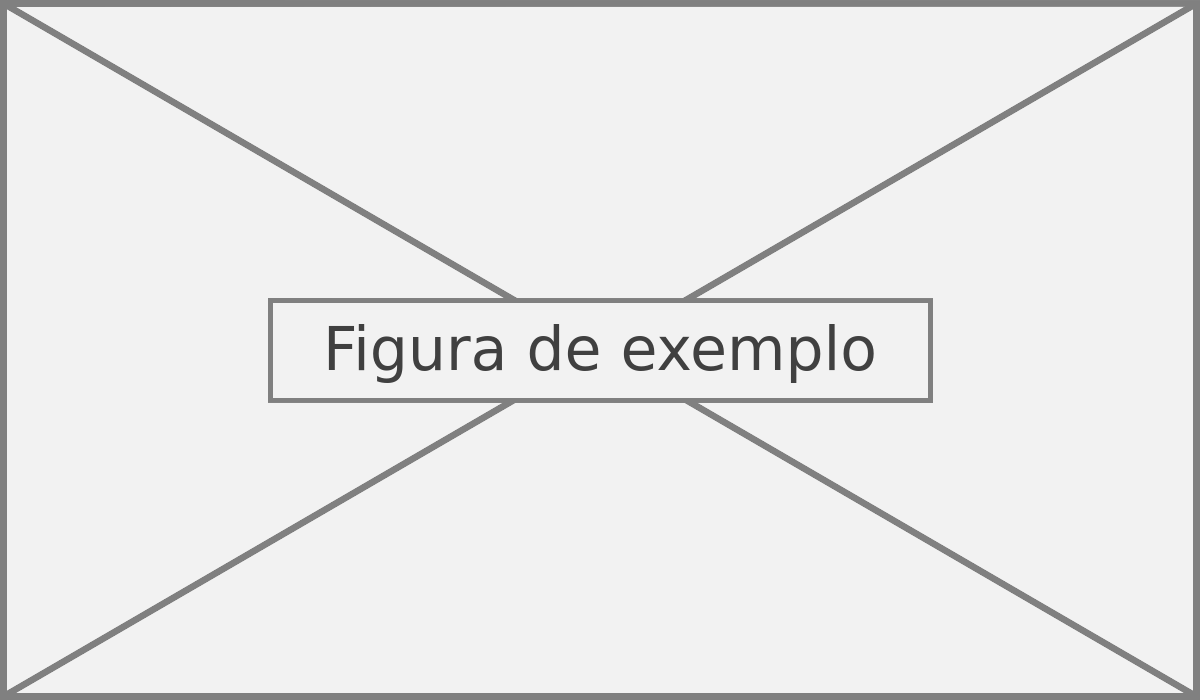
\includegraphics[width=\linewidth]{figuras/exemplo-figura}
		\Fonte{Elaborada pelo autor ([Ano]).}
	\end{minipage}
\end{figure}

\section{Quadros}

% Quadros: conteúdo textual/qualitativo, com bordas fechadas.

O Quadro~\ref{qua:exemplo} apresenta um exemplo de quadro.

\begin{quadro}[htbp]
	\IBGEtab{%
		\caption{Exemplo de quadro}
		\label{qua:exemplo}
	}{%
		\begin{tabular}{|p{4cm}|p{8cm}|}
			\hline
			\textbf{Elemento} & \textbf{Descrição} \\
			\hline
			[Elemento 1] & [Descrição do elemento 1] \\
			\hline
			[Elemento 2] & [Descrição do elemento 2] \\
			\hline
		\end{tabular}%
	}{%
		\Fonte{Elaborado pelo autor ([Ano]).}%
	}
\end{quadro}

	\chapter{Resultados e discussão}
\label{cap:resultados}

[Apresente e discuta os resultados obtidos.]

\section{Tabelas}

% Tabelas (NBR 14724, 5.9, e Normas de Apresentação Tabular do IBGE):
%  - conteúdo numérico;
%  - bordas laterais abertas e traços horizontais apenas no cabeçalho
%    e no fechamento;
%  - título acima e fonte abaixo.

A Tabela~\ref{tab:exemplo} apresenta um exemplo de tabela.

\begin{table}[htbp]
	\IBGEtab{%
		\caption{Exemplo de tabela}
		\label{tab:exemplo}
	}{%
		\begin{tabular}{lccc}
			\toprule
			Categoria & Ano 1 & Ano 2 & Ano 3 \\
			\midrule
			Categoria A & 18 & 24 & 31 \\
			Categoria B & 12 & 17 & 22 \\
			Categoria C &  8 & 14 & 19 \\
			\bottomrule
		\end{tabular}%
	}{%
		\Fonte{Elaborada pelo autor ([Ano]).}%
	}
\end{table}

\section{Notas de rodapé}

Notas de rodapé são impressas em fonte menor e espaço simples\footnote{Exemplo de nota de rodapé.}.

	\chapter{Considerações finais}
\label{cap:conclusao}

[Apresente as conclusões do trabalho, retomando os objetivos, e as sugestões para trabalhos futuros.]


	% Elementos pós-textuais
	\postextual
	\imprimirreferencias{3-pos-textuais/referencias}

	%\imprimirglossario                                        % Opcional

	\imprimirapendices                                          % Opcional
		% Apêndice: texto ou documento elaborado pelo autor, a fim de
% complementar sua argumentação (NBR 14724). Elemento opcional.
% No texto e no sumário: "APÊNDICE A – TÍTULO".
\apendice{Exemplo de apêndice}
\label{ap:A}

[Utilizado quando houver material elaborado pelo próprio autor que seja pertinente ao trabalho, mas que não precise ficar no corpo do texto, como questionários, roteiros de entrevista e instrumentos de coleta de dados.]

		\apendice{Roteiro de entrevista}
\label{ap:B}

\begin{questao}
	\item Pergunta A?
	\item Pergunta B?
		\begin{enumerate}
			\item Opção 1
			\item Opção 2
		\end{enumerate}
	\item Pergunta C?
\end{questao}

		\apendice{Código-fonte}
\label{ap:C}

% Exemplo de código-fonte. Para importar de um arquivo, use:
% \lstinputlisting[language=Python,caption={Descrição}]{caminho/arquivo.py}

\begin{lstlisting}[language=Python,caption={Exemplo de código-fonte em Python}]
def saudacao(nome):
    """Retorna uma saudação."""
    return f"Olá, {nome}!"

print(saudacao("UFERSA"))
\end{lstlisting}

		\apendice{Documento em PDF}
\label{ap:D}

Exemplo de inclusão de um documento em PDF (por exemplo, um formulário elaborado pelo autor).

% Código para inserir todas as páginas de um arquivo PDF:
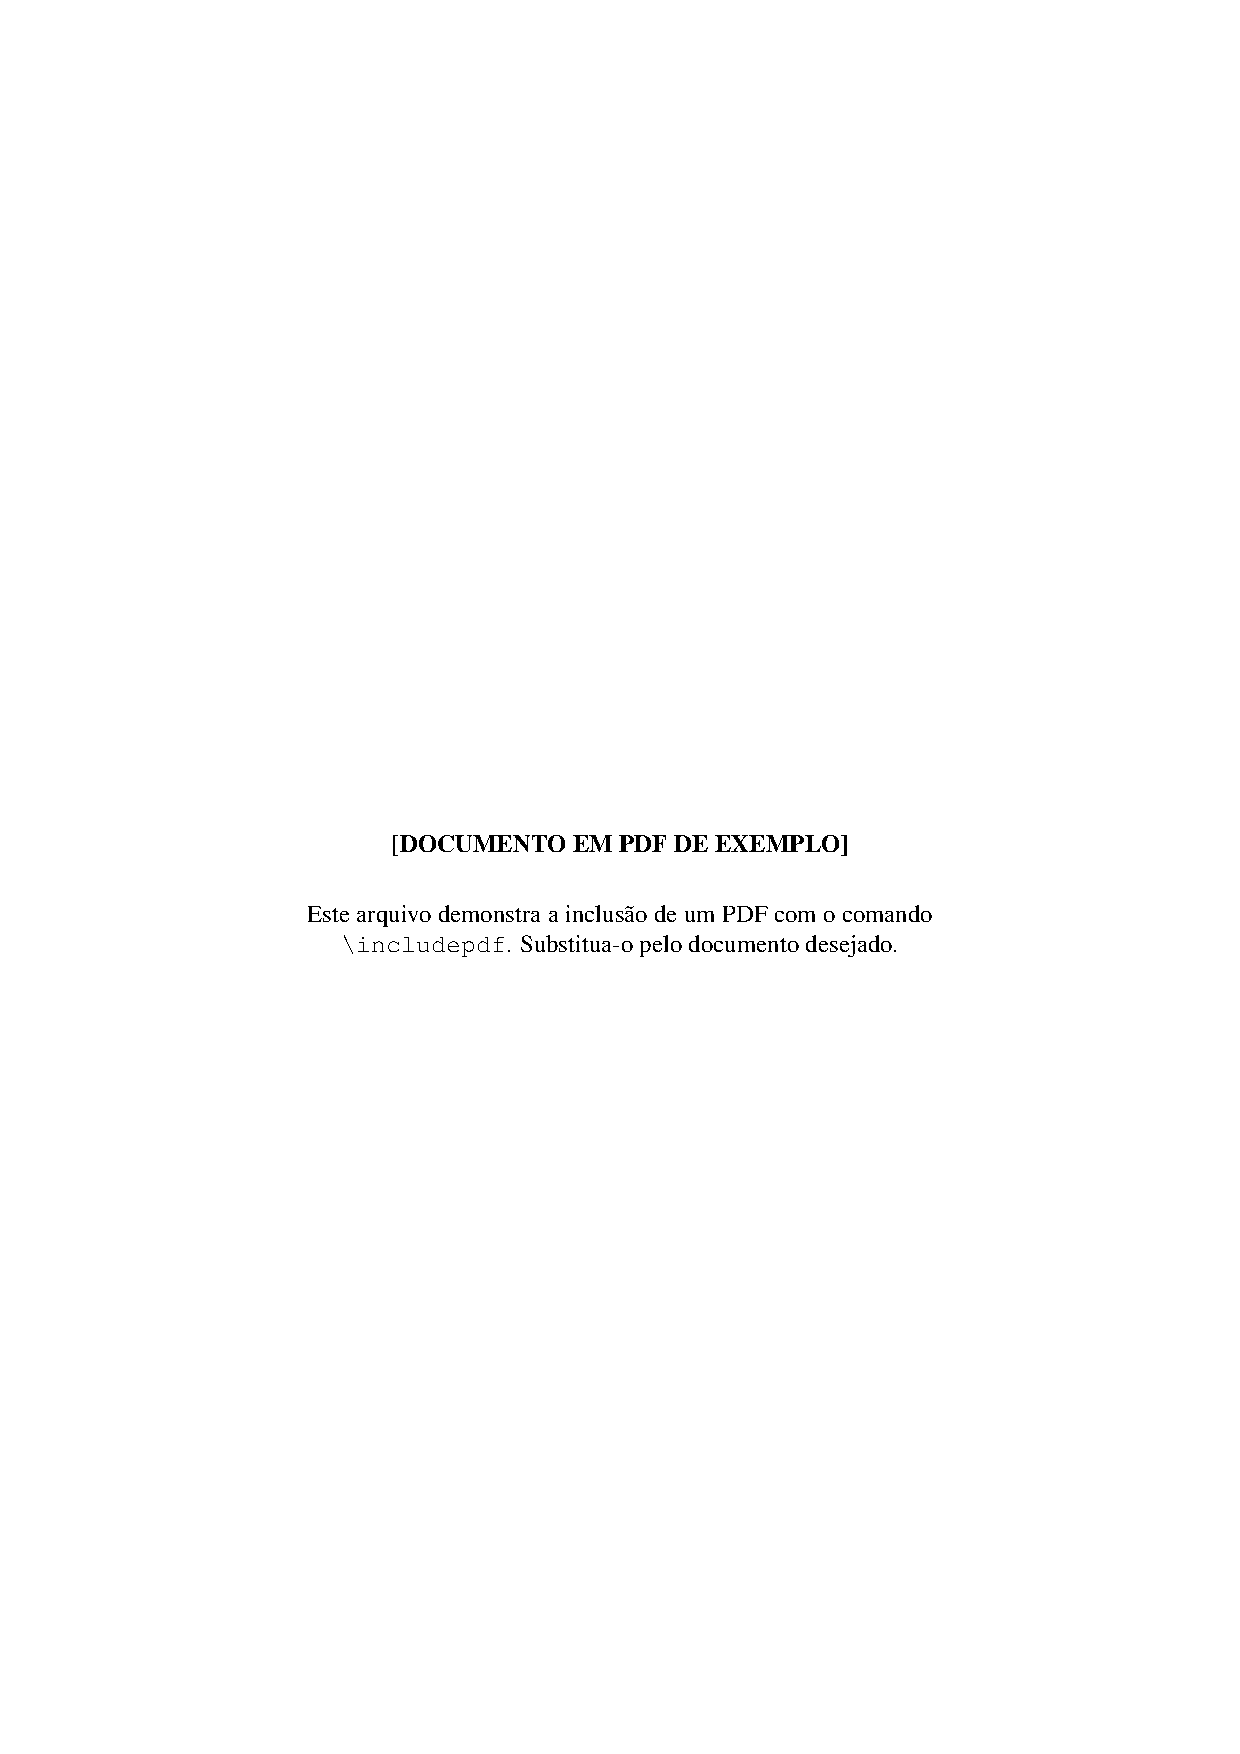
\includepdf[pages={-}]{3-pos-textuais/apendices/exemplo.pdf}


	%\imprimiranexos                                           % Opcional
	%	\anexo{Título do anexo}
	%	Texto ou \includepdf[pages=-]{caminho/do/anexo.pdf}

	%\imprimirindice                                           % Opcional

\end{document}
